%http://www.etaps.org/index.php/2014/cc
%to be submtitted to https://www.easychair.org/account/signin.cgi?timeout=1;conf=cc2014
% abstract: 4th october 2013
% paper: 11th october 2013
%
%Submissions should consist of two parts:
%
%    The first part, at most 4 pages, should describe the tool presented. Please include the URL of the tool (if available) and provide information that illustrates the maturity and robustness of the tool (this part will be included in the proceedings).
%        The second part, at most 6 pages, should explain how the demonstration will be carried out and what it will show, including screen dumps and examples. (This part will be not be included in the proceedings, but will be evaluated.)
%
\documentclass{llncs}

\usepackage{listings}
\usepackage{url}
\usepackage{acronym}
\usepackage{todo}
\usepackage{paralist}
\usepackage[english]{babel}

\usepackage{tikz}
\usetikzlibrary{backgrounds}
\usetikzlibrary{calc}
\usetikzlibrary{positioning}
\usetikzlibrary{shadows}
\usetikzlibrary{arrows}
\usetikzlibrary{shapes}
\usetikzlibrary{fit}

\bibliographystyle{splncs}
\lstset{language=python,morekeywords={cimport, cdef, with},
basicstyle=\ttfamily, keywordstyle=\bf, stringstyle=\color{gray},
captionpos=b}

\acrodef{AST}{Abstract Syntax Tree}
\acrodef{API}{Application Programming Interface}
\acrodef{CLI}{Command Line Interface}
\acrodef{IR}{Internal Representation}
\acrodef{JIT}{Just-In-Time}
\acrodef{AOT}{Ahead-Of-Time}
\acrodef{OO}{Object Oriented}
\acrodef{OSS}{Open Source Software}

\begin{document}
\setcounter{page}{6}


%\maketitle

%\begin{abstract}
%
%    Pythran is a compiler tool that turns source files written in a subset of
%    the Python language into C++11 meta-programs. It also extract from the
%    original source files type annotations used to instantiate the meta-programs
%    into a Python native module that runs typically faster than its interpreted
%    counterpart.
%
%    This paper illustrates the demonstration of Pythran.
%
%\end{abstract}

\section{Tool Paper Motivation}

The purpose of the tool demonstration is to showcase the core functionalities
of the Pythran compiler infrastructure, for three kind of audience:
\begin{inparaenum} \item Python users who want to benefit from the execution
        speed of a compiled language while keeping the advantages of a dynamic,
        high-level language, or who want to prototype C++ code in Python and
        include it in a C++ codebase.  \item Python compiler
        researcher/developers who want to share analyse and passes in a common
    compiler infrastructure.  \item Dynamic language researcher who want to
        explore new or existing optimizations in the context of Python, or want
        to transfer concepts from one language to another.  \end{inparaenum}

To achieve these goal, the presentation relies on \begin{inparaenum} \item User
    stories that illustrates the basic \ac{CLI} of the Pythran compiler,
(\S\ref{sec:cli}).  \item Code snippets related to analyse and passes
    implemented in Pythran (\S\ref{sec:code-analyse},
\S\ref{sec:code-transformation}). \item A sample implementation of parallel map
detection in the Pythran compiler infrastructure (\S\ref{sec:pmap}).  \item
Benchmarks from the \emph{Python Benchmark} codebase that compare several
Python compiler in the context of numerical applications
(\S\ref{sec:python-benchmarks}). \end{inparaenum}

In order to demonstrate the robustness of the tool, the whole presentation
relies on IPython Notebooks, a modern tool that makes it possible to
run code snippets from within the presentation, a feature that helps building
up the confidence in the tool itself. Figure~\ref{fig:notebook} illustrates the
output of a notebook. Input boxes contain code snippet that can be executed
during the presentation, and their output is directly integrated in the
document. This offers a good trade off between interactivity (the audience sees
the code running but the speaker does not to type anything) and reproducibility
(the whole presentation can be executed and check as a test, avoiding the
``demonstration effect'').

\begin{figure}
    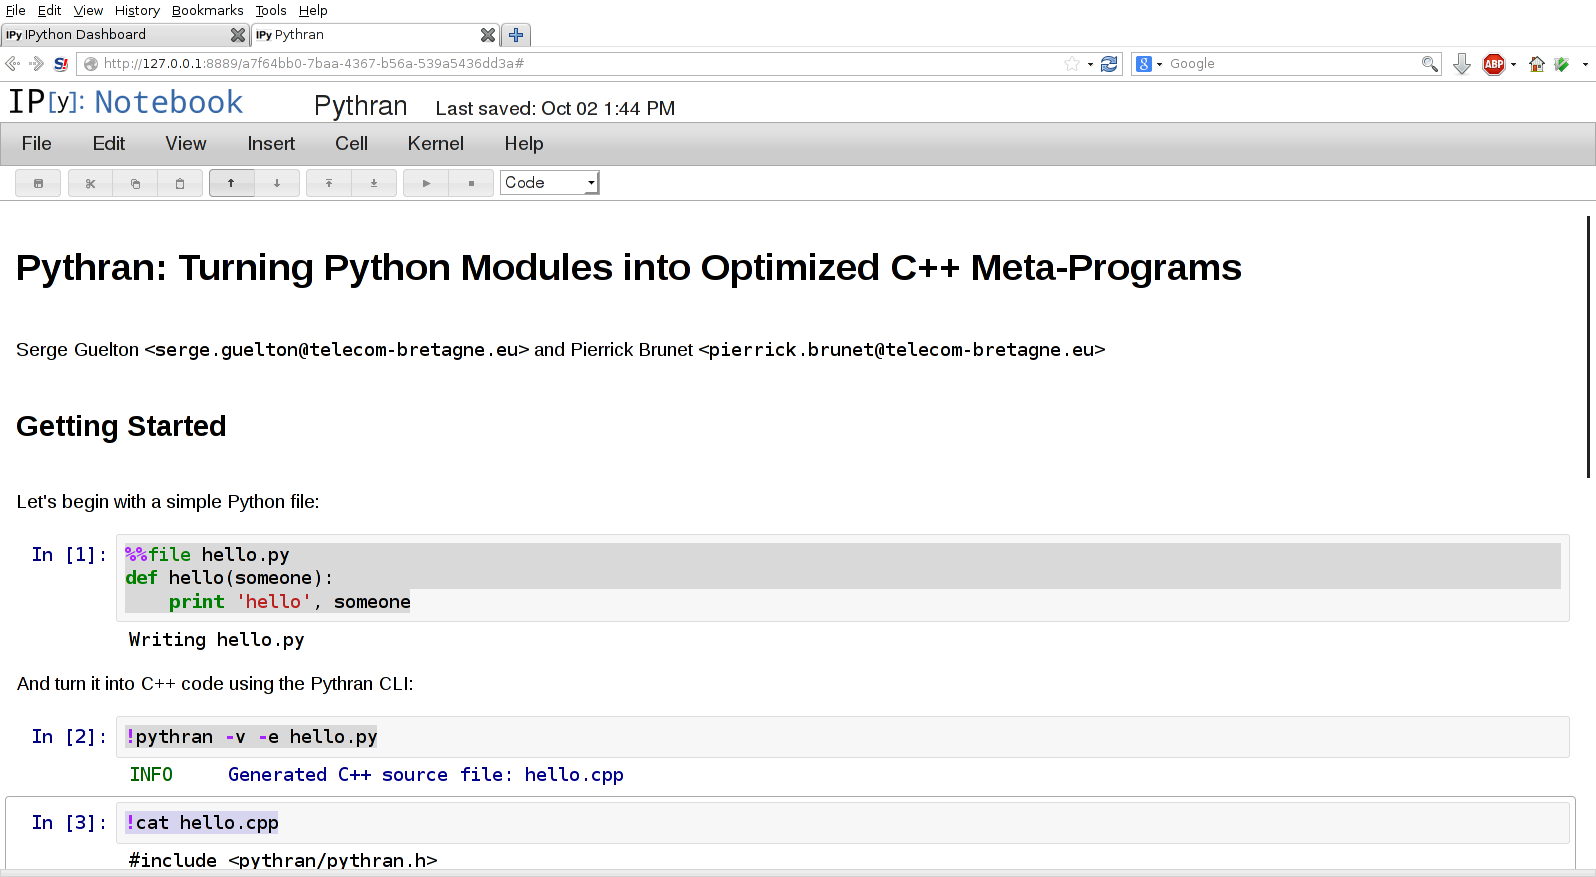
\includegraphics[width=\textwidth]{pythran-notebook}
    \caption{Example of IPython Notebook.}
    \label{fig:notebook}
\end{figure}

%\section*{Conventions}
%
%Python code run from the interpreter is preceded by a triple chevron, but console output is not, as in:
%
%\begin{lstlisting}
%>>> print 7 * 3 * 2
%42
%\end{lstlisting}
%
%Shell code run from the interpreter is preceded by a single chevron, as in:
%\begin{lstlisting}
%> echo graphie
%graphie
%\end{lstlisting}

\section*{Installing Pythran}
\label{sec:install}

Pythran is relatively easy to install. One can rely on the prepackaged version in the Python Package Index, and run:

\begin{lstlisting}
> pip install pythran
\end{lstlisting}

A Debian package is also available, so after a slight modification of \texttt{sources.list} (see \url{http://ridee.enstb.org/debian/info.html}):

\begin{lstlisting}
> sudo apt-get install pythran
\end{lstlisting}


Compilation from sources starts is the best way to get last modifications:

\begin{lstlisting}
> git clone https://github.com/serge-sans-paille/pythran
> cd pythran && python setup.py install
\end{lstlisting}

Pythran-generated binaries depend on \texttt{libboost-python} for interfacing
Python with C++, \texttt{libgmpxx} for multi precision arithmetic, and a modern
C++11 compiler (clang version 3.4 or g++ version 4.8).

\section{Pythran \acf{CLI}}
\label{sec:cli}

Pythran is a source-to-source compiler that turns Python code into C++ meta
programs then instantiate it for given types and compile it to a native module
that can be imported using Python native module import.

\subsection{Python to C++ Conversion}

Let us consider a very simple module, \texttt{hello.py}:

\begin{lstlisting}
def hello(name):
    print 'hello', name
\end{lstlisting}

Pythran can turn it into a pure C++ source file:

\begin{lstlisting}
> pythran -e hello.py -o hello.hpp
> cat hello.hpp
#include <pythran/pythran.h>
namespace __pythran_hello {
  struct hello {
    typedef void callable;
    template <typename argument_type0 >
    struct type {
        typedef typename assignable<
          typename std::remove_cv<
            typename std::remove_reference<
              decltype(__builtin__::None)
            >::type
          >::type
        >::type result_type;
    }; 
    template <typename argument_type0 >
    typename type<argument_type0>::result_type
    operator()(argument_type0 const &) const;
  };
  template <typename argument_type0 >
  typename hello::type<argument_type0>::result_type
  hello::operator()(argument_type0 const & name) const {
    print(core::string("hello"), name);
    return __builtin__::None;
  }
}
\end{lstlisting}

Generated header code contains two parts: \begin{inparaenum} \item A meta class
\texttt{hello} that reflects the Python function, \item a templated nested
class \texttt{type} that contains the type inference logic. \end{inparaenum}

The header can be instantiated from regular C++ code, and template argument
detection emulates Python duck typing:

\begin{lstlisting}
> cat hello.cpp
#include "hello.hpp"
using namespace __pythran_hello;
int main() {
  hello h;
  h("world"); h(42);
  return 0;
}
> cxx -std=c++11 -I... hello.cpp -o hello
> ./hello
hello world
hello 42
\end{lstlisting}

\subsection{Python to Native Module Conversion}

To turn a Python module into a native module, Pythran needs type information
concerning the module interface. These type informations are provided by the
user in the form of comments, as in:

\begin{lstlisting}
#pytrhan export hello(str)
#pytrhan export hello(int)
def hello(name):
    print 'hello', name
\end{lstlisting}

These type annotations are used by the Pythran compiler to automatically
instanciate the generated C++ meta program and generate the Python foreign
interface glue. The associated code can be inspected using:

\begin{lstlisting}
> pythran -E hello.py
\end{lstlisting}

\noindent or directly compiled using:

\begin{lstlisting}
> pythran -O2 -g hello.py
\end{lstlisting}

Note that any compiler flags not relevant to Pythran is forwarded to the C++
compiler. the defaults are parametrized through a user configuration file
\texttt{.pythranrc} and its system-wide counterpart.

\section{Python Code Analysis in Pythran}
\label{sec:code-analyse}

Pythran does not only perform Python-to-C++ translation. It also applies
several high-level optimizations backed up by several code analyse.

One such analysis is the argument effect analysis. Informally, the analyse
traverses the \ac{IR} in a per function basis, building intra-function
argument effects as well as an inter-function dependency graph, then performs a
flooding pass over the dependency graph to compute a inter-procedural argument
effects. One can observe the result of this analyse using the \texttt{pythran} module:

\begin{lstlisting}
>>> from pythran import passmanager, analysis
>>> pm = passmanager.PassManager("tutorial_module")
>>> code = '''
def foo(l,a):
  l+=[a]
def bar(g):
  foo(g, 1)'''
>>> tree = ast.parse(code)
>>> ae = pm.gather(analysis.ArgumentEffects, tree)
>>> foo, bar = tree.body
>>> ae[foo]
[True, False]
>>> ae[bar]
[True]
\end{lstlisting}

Pythran also implements an intra-procedural aliasing analysis that provides
critical piece of informations:

\begin{lstlisting}
>>> code = '''
def foo(c, d):
    b= c or d
    return b'''
>>> tree = ast.parse(code)
>>> al = pm.gather(analysis.Aliases, tree)
>>> returned = tree.body[-1].body[-1].value
>>> print ast.dump(returned)
Name(id='b', ctx=Load())
>>> sorted(a.id for a in al[returned].aliases)
['c', 'd']
\end{lstlisting}


\section{Python Code Transformation in Pythran}
\label{sec:code-transformation}

Pythran provides two kind of passes: passes that transform Python's \ac{AST}
into Pythran \ac{IR}, and optimizations passes. An example of \ac{AST} to
\ac{IR} transformation is \emph{destructuring}

\begin{lstlisting}
>>> from pythran import passes
>>> tree = ast.parse("a, b = 1, 3.5")
>>> pm.apply(passes.NormalizeTuples, tree)
>>> print pm.dump(backend.Python, tree)
if 1:
    __tuple10 = (1, 3.5)
    a = __tuple10[0]
    b = __tuple10[1]
\end{lstlisting}

Among available optimizations, Pythran can use a variant of \emph{deforestation}, as showcased in the following snippet:
\begin{lstlisting}
>>> code = '''
def norm(l):
  return sum(n*n for n in l)'''
>>> tree = ast.parse(code)
>>> pm.apply(optim.GenExpToImap, tree)
>>> print pm.dump(backend.Python, tree)
import itertools
def norm(l):
    return sum(itertools.imap((lambda n: (n * n)), l))
\end{lstlisting}

\section{Live Exercise: Implement Parallel Map Detection in Pythran}
\label{sec:pmap}

Pythran makes it fairly easy to add new analyse that depend from existing
analyse. Let us take the example of parallel map detection. First step consist
in declaring a new analysis, that works at the function level:

\begin{lstlisting}
class ParallelMaps(ModuleAnalysis):
\end{lstlisting}

Then one need to list the analyse this analysis depends on:
\texttt{PureFunctions} to detect pure functions and \texttt{Aliases} to use
alaising informations:

\begin{lstlisting}
  def __init__(self):
    self.result = set()
    super(ParallelMaps, self).__init__(PureFunctions, Aliases)
\end{lstlisting}

The \texttt{result} member variable is used to store the result of the
analysis. Next one need to inspect each function call, select those calling the
\texttt{map} builtin and verify the first argument always aliases to a pure
function:

\begin{lstlisting}
  def visit_Call(self, node):
    if all(alias == modules['__builtin__']['map']
           for alias in self.aliases[node.func].aliases):
      if all(self.pure_functions.__contains__(f)
             for f in self.aliases[node.args[0]].aliases):
        self.result.add(node)
\end{lstlisting}

Matching calls are stored as the result of the analyse.

\section{Python Benchmarks Project}
\label{sec:python-benchmarks}

Python Benchmarks is a project that aims at comparing the existing approaches to
speedup numerical computations in Python. The project and its result can be
found on \url{https://github.com/numfocus/python-benchmarks}.
Figure~\ref{fig:python-benchmarks} illustrates the result of one of the
benchmark, showing that Pythran performs well compared to existing approaches.

\begin{figure}

    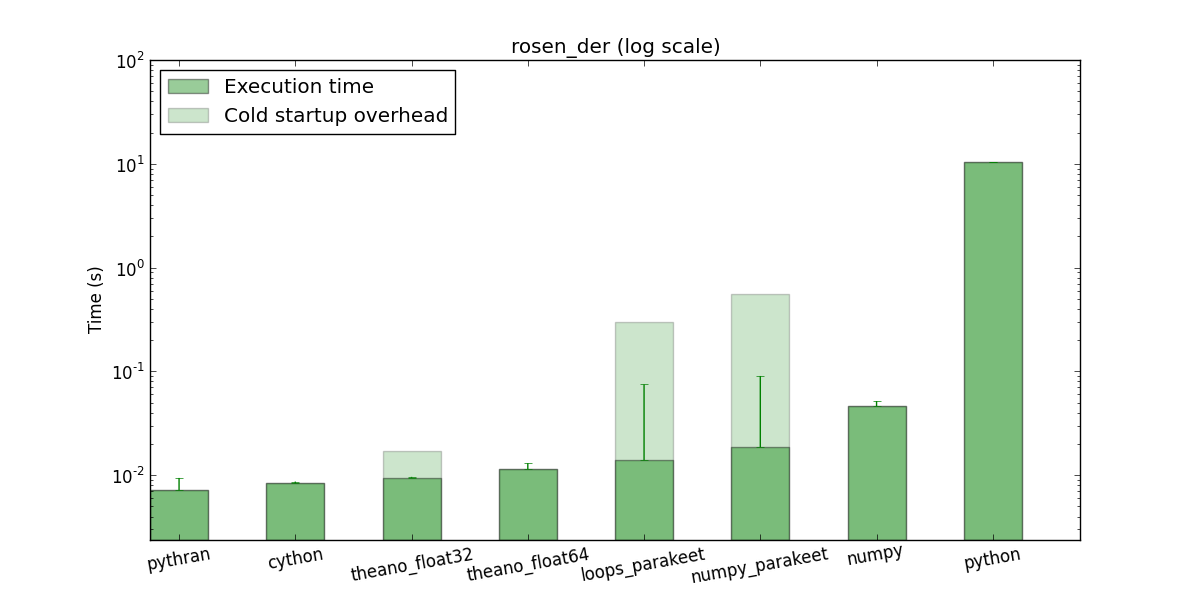
\includegraphics[width=\textwidth]{rosen_der_logscale}
    \caption{Timings for the \texttt{rosen\_der} function from Python Benchmarks.}
    \label{fig:python-benchmarks}

\end{figure}

\section{Conclusion}

The Pythran compiler is an open source project that offers a compilation
infrastructure to analyze and optimize a large class of Python programs.
Benchmarks shows it can produce C++ code whose performance match those of
annotated or JIT compiled code, and it is mature enough to host third part
contributions.

\end{document}
